\chapter{Các kiến thức nền tảng và nghiên cứu liên quan}
Chương này sẽ trình bày về một số kiến thức nền tảng như: trình biên dịch, trình dịch ngược, một số kỹ thuật thường được sử dụng trong trình dịch ngược và kiến trúc của trình dịch ngược Boomerang. Việc vì sao lựa chọn trình dịch ngược Boomerang để hiện thực các giải pháp cho bài toán cũng sẽ được bàn đến trong chương này. \\
\section{Trình biên dịch}
Trình biên dịch (compiler) là một chương trình hoặc một bộ chương trình máy tính, có nhiệm vụ biến đổi mã nguồn được viết bằng một ngôn ngữ lập trình này (ngôn ngữ lập trình gốc) sang một ngôn ngữ lập trình khác (ngôn ngữ lập trình đích), thường sẽ có dạng nhị phân và thực thi được. \\
Các bước của trình biên dịch gồm có:
\begin{itemize}
	\item Phân tích từ vựng (lexical analysis): Đây là quá trình chuyển hóa một chuỗi các ký tự (ví dụ như các câu lệnh trong một chương trình máy tính) thành chuỗi các từ tố (token), ví dụ như: định danh, số nguyên, số thực... Giai đoạn này kiểm tra các lỗi về từ vựng, chính tả của chương trình. \\
	
	Trong hình \ref{fig:lexi}, các ký tự \textit{a}, \textit{b} được nhận diện là các định danh (identifier), \textit{10} được nhận diện là số nguyên (integer), \textit{=} và \textit{+} được nhận diện là các phép tính (operator), \textit{;} là ký tự đặc biệt kết thúc một câu lệnh.
	
	\begin{figure}[h]
		\centering
		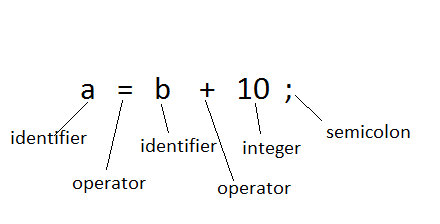
\includegraphics{fig21.png}
		\caption{Phân tích một câu lệnh thành các token}
		\label{fig:lexi}
	\end{figure}
	
	\item Phân tích cú pháp (syntax analysis): Từ chuỗi các từ tố được tạo ra ở giai đoạn trên, một chương trình gọi là parser sẽ tạo ra một cấu trúc dữ liệu, thường là parse tree hoặc abstract syntax tree. Giai đoạn này sẽ kiểm tra các lỗi về cấu trúc ngữ pháp.
	
	Câu lệnh gán từ ví dụ trên sẽ được phân tích thành cây cấu trúc như hình \ref{fig:parser}
	
	\begin{figure}[h]
		\centering
		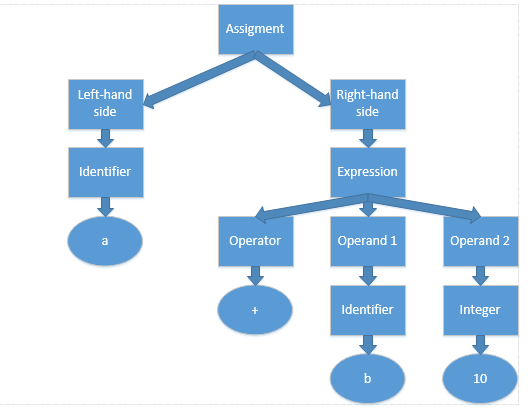
\includegraphics{fig22.png}
		\caption{Cây cấu trúc cho một câu lệnh gán}
		\label{fig:parser}
	\end{figure}
	
	\item Phân tích ngữ nghĩa (sematic analysis): Trong giai đoạn này, từ cây cấu trúc đã có, trình biên dịch sẽ áp dụng các luật về ngữ nghĩa để kiểm tra tính đúng đắn của chương trình. Thường sẽ là các luật về kiểu dữ liệu, kiểm tra tầm vực của biến và object binding.\\
	Tiếp tục ví dụ ở trên, trong gian đoạn này, trình biên dịch sẽ kiểm tra xem các biến \textit{a} và \textit{b} đã được khai báo chưa, tầm vực của các biến có phủ tới vị trí của câu lệnh không (ví dụ: có những biến được khai báo ở hàm \textit{A} thì sẽ không có tầm vực ở bên ngoài hàm \textit{A}), kiểu của biến có phù hợp với câu lệnh gán không (ví dụ: nếu \textit{b} có kiểu là \textbf{string} thì câu lệnh trên không hợp lệ).
	\begin{figure}[h]
		\centering
		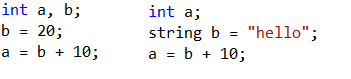
\includegraphics{fig23.png}
		\caption{Ví dụ về lỗi kiểu biến}
		\label{fig:semerror}
	\end{figure}
	
	Trong hình \ref{fig:semerror}, cả hai đoạn mã đều hợp lệ tính đến cuối giai đoạn phân tích cú pháp. Tuy nhiên, giai đoạn phân tích ngữ nghĩa sẽ phát hiện ra đoạn mã ở bên phải không hợp lệ vì nó vi phạm các ràng buộc về kiểu.
	
	\item Tạo ra mã trung gian: Sau khi trải qua các giai đoạn phân tích và kiểm tra, trình biên dịch sẽ tiến hành sinh mã trung gian từ mã nguồn. Đặc điểm của mã trung gian là đơn giản và rất gần với mã đích, tuy nhiên con người vẫn có thể đọc và hiểu được. Việc sinh mã trung gian nhằm giảm thiểu chi phí cho trình biên dịch khi phải sinh mã đích cho nhiều kiến trúc máy khác nhau. Thay vì với mỗi kiến trúc máy, trình biên dịch phải tạo ra công cụ riêng để dịch từ mã nguồn sang mã đích, thì ở đây chỉ cần tạo ra công cụ để dịch từ mã trung gian - vốn đã rất gần với mã đích.\\
	
	
	\item Tạo mã đích: Từ mã trung gian, tùy vào kiến trúc máy sẽ thực thi chương trình, trình biên dịch sẽ tạo ra mã đích tương ứng. Giai đoạn này sẽ thực hiện các công việc như: lựa chọn câu lệnh trung gian sẽ thực hiện, quyết định các giá trị được lưu trong thanh ghi, sắp xếp thứ tự thực hiện các câu lệnh. Đầu ra của giai đoạn là mã máy có thể thực thi được.
	
	
	\item Tối ưu mã đích: Để tăng tốc độ thực hiện chương trình cũng như giảm các chi phí chạy chương trình, giai đoạn tối ưu mã đích sẽ kiểm tra và áp dụng các kỹ thuật nhằm loại bỏ mã chết, tối ưu vòng lặp, loại bỏ dư thừa... Giai đoạn này không nhất thiết chỉ thực hiện ở cuối quá trình biên dịch mà có thể nằm ở bất cứ đâu.
\end{itemize}

\section{Trình dịch ngược}
Mục tiêu của trình dịch ngược là chuyển đổi chương trình được viết bằng một ngôn ngữ cấp thấp (thường là mã máy) lên một ngôn ngữ cấp cao hơn (như C, C++...). Vì vậy, trình dịch ngược (decompiler) có thể xem như một quá trình đảo ngược của trình biên dịch (compiler). Chương trình đầu ra phải thực hiện được những chức năng tương đương như chương trình đầu vào. \\

\begin{figure}[h]
	\centering
	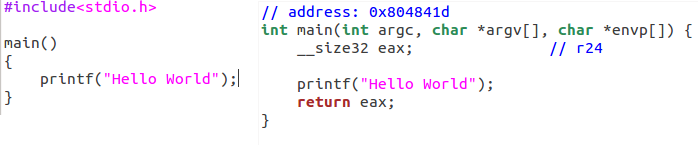
\includegraphics{fig24.png}
	\caption{Đoạn mã gốc và đoạn mã được dịch ngược bởi trình dịch ngược Boomerang}
\end{figure}

Qúa trình dịch ngược có thể chia thành các giai đoạn sau:
\begin{itemize}
	\item Loader: Load file cần dịch ngược, đọc từ file ra các thông tin như: loại file, loại kiến trúc máy... và xác định được ngõ vào của chương trình (tương đương với hàm main trong C).
	\item Disassembly: Mã gốc sẽ được chuyển thành mã trung gian, mã trung gian là gì thì tùy vào trình dịch ngược. Ví dụ Boomerang sẽ dùng mã trung gian là Register Transfer Language.
	\item Analysis: Sau khi đã chuyển sang mã trung gian, chương trình sẽ đi qua các bước phân tích để khôi phục lại thông tin đã mất trong quá trình biên dịch. Các phân tích thường phải có là: lan truyền biểu thức, loại bỏ mã chết, xác định nguyên mẫu hàm (function prototype), xác định kiểu dữ liệu...
	\item Code generation: Trải qua các kỹ thuật phân tích để xác định được thông tin cần thiết về dữ liệu, kiểu và luồng điều khiển chương trình, giai đoạn cuối cùng của dịch ngược là sinh ra mã chương trình bằng ngôn ngữ bậc cao. 
\end{itemize}
\begin{figure}[h]
	\centering
	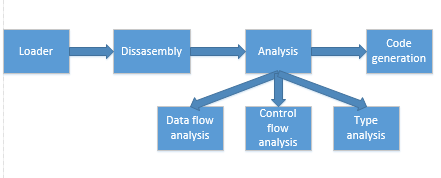
\includegraphics{fig27.png}
	\caption{Các bước cơ bản của một trình dịch ngược}
\end{figure}
\section{Một số kỹ thuật tiêu biểu được sử dụng trong các công cụ dịch ngược}
\subsection{Lan truyền biểu thức}
Lan truyền biểu thức (Expression propagation) là biến đổi phổ biến nhất trong quá trình dịch ngược một đoạn code. Nguyên tắc truyền biểu thức cũng rất đơn giản: Với các câu lệnh sử dụng giá trị của một biến nào đó, ta có thể thay tên biến đó bằng biểu thức nằm bên phải câu lệnh gán biến đó.\\
\begin{figure}[h]
	\centering
	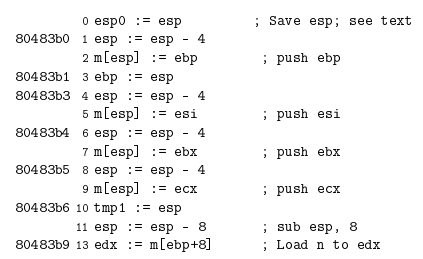
\includegraphics{fig33.png}
	\caption{Một đoạn mã trước khi thực hiện lan truyền biểu thức}
	\label{fig:33}
\end{figure}
\begin{figure}[h]
	\centering
	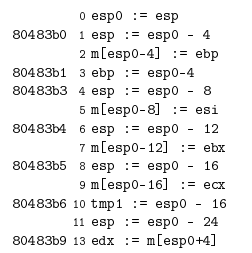
\includegraphics{fig34.png}
	\caption{Đoạn mã ở hình \ref{fig:33} sau khi thực hiện lan truyền biểu thức}
	\label{fig:34}
\end{figure}
Hình \ref{fig:33} và \ref{fig:34} là một ví dụ cho lan truyền biểu thức. Trong hình \ref{fig:33}, ta có các câu lệnh ở dạng mã trung gian trước khi thực hiện lan truyền biểu thức. Hình \ref{fig:34} là kết quả sau khi thực hiện lan truyền biểu thức. Ở đây ta giả sử có một biến đặc biệt là \textit{esp0} được gán giá trị là giá trị ban đầu của biến \textit{esp}. Ta sẽ thực hiện một thay thế đặc biệt ở câu lệnh số 1, thay vế phải của câu lệnh gán này - \textit{esp} - bằng biến tương đương với nó là \textit{esp0}. Sau đó, ở các câu lệnh tiếp theo, ta sẽ tiếp tục thay thế biến \textit{esp} bằng các biểu thức tương đương. Ví dụ: Ở câu lệnh số 2, biểu thức tương đương của \textit{esp} là \textit{esp0 - 4}, còn ở câu lệnh số 5, biểu thức tương đương của \textit{esp} là \textit{esp0 - 8} (do \textit{esp} đã được gán một giá trị mới ở câu lệnh số 4). Tuy nhiên, biểu thức \textit{esp0 - 8} không thể được dùng để thay thế cho biến \textit{esp} ở câu lệnh số 7 được, vì lúc đó \textit{esp} đã mang giá trị khác.\\

Như vậy, qua ví dụ trên, ta có thể thấy việc lan truyền biểu thức từ câu lệnh \textit{a} có dạng \textit{x := exp} đến một câu lệnh \textit{b} chỉ có thể được thực hiện nếu đáp ứng hai điều kiện sau:

\begin{itemize}
	\item \textit{a} phải là câu lệnh gán có vế trái là \textit{x} ở gần \textit{b} nhất. Nói cách khác, giữa \textit{a} và \textit{b} không được có bất cứ câu lệnh gán nào khác có vế trái là \textit{x}
	\item Trên tất cả các luồng đi của chương trình từ \textit{a} tới \textit{b}, không có câu lệnh gán nào có vế trái là bất kỳ biến nào được sử dụng trong \textit{a}
\end{itemize}
\begin{figure}[h]
	\centering
	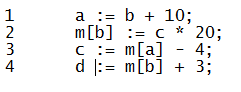
\includegraphics{fig35.png}
	\caption{Đoạn mã trung gian với bốn câu lệnh gán đơn giản}
	\label{fig:35}
\end{figure}
Ở đoạn code hình \ref{fig:35}, ta có thể thực hiện lan truyền biểu thức với biến \textit{a} ở câu lệnh số 3, kết quả sẽ là \textit{c := m[b + 10] - 4;} và câu lệnh gán biến \textit{a} sẽ được loại bỏ bằng kỹ thuật loại bỏ mã chết được bàn ở phần tiếp theo. Tuy nhiên, ta không thể thực hiện lan truyền biểu thức với \textit{m[b]} ở câu lệnh số 4, vì biến \textit{c} được sử dụng trong câu lệnh gán số 2 đã được sử dụng làm vế trái trong câu lệnh gán số 3.\\

Với mã trung gian như trên, để kiểm tra hai điều kiện thỏa mãn việc lan truyền biểu thức phải mất rất nhiều thời gian, ta phải xét hết tất cả các luồng chương trình từ câu lệnh gán đến câu lệnh sử dụng biến, kiểm tra tất cả các biến được sử dụng trong câu lệnh gán. Tuy nhiên, với mã SSA - sẽ được nói đến ở mục \ref{ssa}, hai điều kiện trên sẽ được tự động thỏa mãn và không cần bất kỳ kiểm tra gì thêm.
\subsection{Loại bỏ mã chết}

Mã chết bao gồm các câu lệnh gán mà biến ở vế trái của nó không bao giờ được dùng. Cần phân biệt mã chết (dead code) với mã không bao giờ được chạy (unreachable code), là những câu lệnh mà không có bất kỳ luồng điều khiểu hợp lệ nào của chương trình đi qua (ví dụ: câu lệnh ở dưới một vòng lặp vô hạn). Việc lan truyền biểu thức sẽ dẫn đến việc có một số biến không được sử dụng, từ đó sinh ra mã chết. \\
Từ đoạn mã đã được lan truyền biểu thức ở hình \ref{fig:34}, ta thấy biến \textit{esp} không được sử dụng ở bất kỳ câu lệnh nào. Vì vậy, các câu lệnh gán có \textit{esp} ở vế trái sẽ được xem là mã chết và được loại bỏ. Kết quả là hình \ref{fig:36}.

\begin{figure}[h]
	\centering
	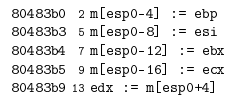
\includegraphics{fig36.png}
	\caption{Đoạn mã ở hình \ref{fig:35} sau khi loại bỏ mã chết}
	\label{fig:36}
\end{figure}

Để kiểm tra xem một biến có được sử dụng hay không, ta phải xem xét tất cả các luồng chạy hợp lệ của chương trình từ câu lệnh gán biến đến cuối chương trình, điều này phức tạp và mất nhiều thời gian. Tuy nhiên, mã SSA sẽ giúp việc kiểm tra mã chết dễ dàng hơn.
\subsection{Mã SSA} \label{ssa}

Mã SSA là một dạng mã trung gian có tính chất là: Mỗi biến hoặc vùng nhớ được định nghĩa duy nhất một lần trong toàn bộ chương trình. \\

Để chuyển từ mã RTL sang mã SSA, các biến cần phải được thay đổi tên, thường là sẽ được đánh số thứ tự đằng sau tên biến gốc. Ví dụ, nếu biến \textit{a} xuất hiện ở vế trái của 3 câu lệnh gán, thì sẽ được đánh số lần lượt là \textit{a1}, \textit{a2} và \textit{a3} như ví dụ ở hình \ref{fig:38}

\begin{figure}[h]
	\centering
	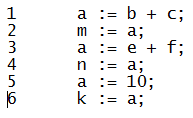
\includegraphics{fig37.png}
	\caption{Đoạn mã trung gian với 3 lần định nghĩa biến \textit{a}}
	\label{fig:37}
\end{figure}

\begin{figure}[h]
	\centering
	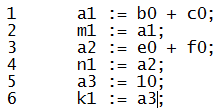
\includegraphics{fig38.png}
	\caption{Đoạn mã ở hình \ref{fig:38} đã được chuyển sang dạng mã SSA}
	\label{fig:38}
\end{figure}

Với tính chất của mã SSA, việc lan truyền biểu thức và loại bỏ mã chết sẽ được hiện thực rất dễ dàng.\\

Đối với lan truyền biểu thức, hai điều kiện đã được tự động thỏa mãn. Điều kiện đầu tiên thỏa mãn vì mỗi biến đều được định nghĩa duy nhất một lần, không có việc có nhiều định nghĩa cho cùng một tên biến (nếu ở mã gốc có việc đó, thì khi chuyển sang mã SSA, biến đó sẽ được đánh số để trở thành những biến khác nhau ở mỗi câu lệnh gán). Điều kiện thứ hai thỏa mãn vì chắc chắn từ câu lệnh gán một biến đến bất kỳ câu lệnh nào sử dụng biến đó, biến sẽ không được định nghĩa lại.\\

Việc loại bỏ mã chết cũng có thể thực hiện dễ dàng nhờ vào hành động thu thập thông tin về định nghĩa và sử dụng của một biến. Trong quá trình biến đổi từ mã RTL sang SSA, ta có thể xây dựng nên một bảng vị trí câu lệnh gán của một biến và vị trí các câu lệnh sử dụng biến đó. Trải qua các quá trình phân tích, nhất là lan truyền biểu thức, bảng này sẽ được cập nhật lại. Đến cuối cùng, các biến được định nghĩa nhưng không được sử dụng ở bất kỳ câu lệnh nào sẽ được xác định và loại bỏ các câu lệnh gán dư thừa đi.\\

\section{Tình hình phát triển trình dịch ngược hiện nay}
\label{sec:whyboom}
Hiện nay, có rất nhiều trình dịch ngược đã và đang được phát triển. Hầu hết đều hỗ trợ việc dịch ngược từ mã máy và có thể chia làm hai loại: trình dịch ngược nhận đầu vào là mã máy chạy trên máy ảo (ví dụ: mã máy được dịch từ các chương trình viết bằng Java, C\#) và trình dịch ngược nhận đầu vào là mã máy chạy trên máy thật. Loại thứ nhất có số lượng nhiều hơn, lý do có thể vì mã máy ảo còn lưu giữ được khá nhiều thông tin từ chương trình gốc, điển hình như tên biến toàn cục (xem hình \ref{fig:ilspy}). Vì vậy, bài toán cần giải quyết để xây dựng một trình dịch ngược dạng này không nhiều. Ngược lại, mã máy thật đã bị mất hầu hết các thông tin từ chương trình gốc, nên việc khôi phục thông tin ở các trình dịch ngược từ mã máy thật khá phức tạp. Trong hình \ref{fig:boomerang}, tên biến ở chương trình gốc đã bị mất đi. Ngoài ra, cấu trúc vòng lặp cũng thay đổi từ \textit{for} sang \textit{while}. Đó là do ở mã máy, cấu trúc vòng lặp ở ngôn ngữ cấp cao đã được dịch thành các câu lệnh kiểm tra điều kiện và jump, nên Boomerang phải sử dụng các thuật toán phân tích luồng điều khiển để tạo ra cấu trúc vòng lặp mới, đôi khi có thể không trùng khớp với cấu trúc vòng lặp ban đầu.

\begin{figure}[h]
	\centering
	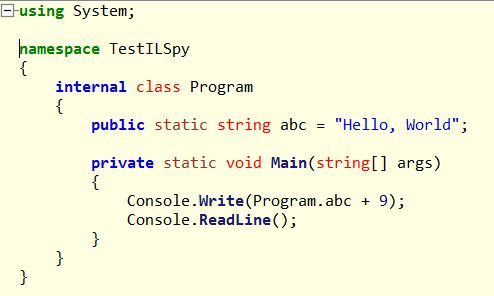
\includegraphics{fig25.png}
	\caption{Một đoạn mã được dịch ngược bởi trình dịch ngược ILSpy. Tên biến static \textit{abc} được giữ nguyên như mã gốc}
	\label{fig:ilspy}
\end{figure}
\begin{figure}[h]
	\centering
	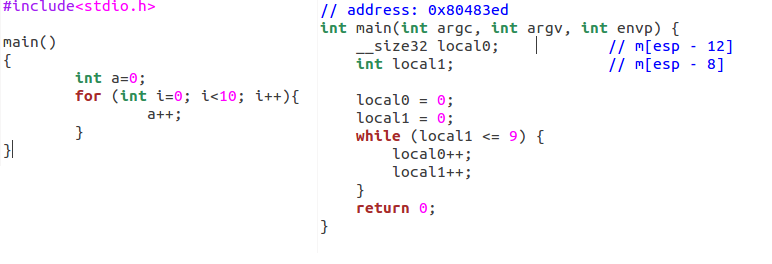
\includegraphics{fig26.png}
	\caption{Một đoạn mã được dịch bởi Boomerang}
	\label{fig:boomerang}
\end{figure}

Một số trình dịch ngược phổ biến có thể kể đến là:

\begin{itemize}
	\item dcc: Là một trình dịch ngược từ mã máy, đây được xem là một trong những trình dịch ngược đầu tiên và vẫn còn được phát triển tới bây giờ.
	\item ILSpy: Là một trình dịch ngược cho .NET, input là các file assembly được dịch từ chương trình .NET, được phát triển bởi isharpcode. Hiện nay ILSpy vẫn đang được tiếp tục phát triển và thêm các tính năng mới.
	\item Procyon: Là một trình dịch ngược cho Java. Trước đây lựa chọn hàng đầu để dịch ngược mã Java là JAD (Java decompiler), tuy nhiên hiện nay JAD đã ngừng phát triển và mã nguồn không còn mở nữa. Một số trình dịch ngược khác được phát triển và Procyon là một đại diện tiêu biểu.
	\item Boomerang: Là trình dịch ngược từ mã máy, mục tiêu là tạo ra một trình dịch ngược không quan tâm tới ngôn ngữ viết ra chương trình gốc. Boomerang đã ngừng phát triển từ năm 2006 do hai lập trình viên chính bắt đầu làm việc cho một công ty mà lĩnh vực nghiên cứu của họ trùng lặp với Boomerang.
\end{itemize}

Trong số các trình dịch ngược nêu trên, cần tìm ra trình dịch ngược phù hợp nhất để làm nền tảng cho việc hiện thực những giải pháp mà luận văn đề ra. Để tìm ra trình dịch ngược đó, phải có sự phân tích, đánh giá sự phù hợp của những trình dịch ngược thông qua một số tiêu chí. Phần đánh giá này được thể hiện ở bảng \ref{table:table1}
\begin{table}[h!]
	\centering
	\begin{tabular}{ |p{0.7cm}| p{2cm}| p{1.5cm}| p{1.5cm}| p{2cm}| p{1.5cm}| p{1.5cm}
			| p{1.5cm}| p{1.5cm}| p{1.5cm}| }
	\hline
		STT & Tên trình dịch ngược & Phù hợp với bài toán cần giải quyết & General compiler & Mã máy lưu trữ được nhiều thông tin gốc của chương trình & Có người hỗ trợ & Có tài liệu đầy đủ & Viết bằng ngôn ngữ quen thuộc & Tổng điểm\\
		\hline
		1 & Boomerang & 1 & 1 &0 & 5 & 2 & 0 & 9\\
	\hline
		2 & ILSpy & 0 & 0 & 2 & 0& 3 & 2 & 7\\
		\hline
		3 & dcc & 0 &1&0&0&0&0&1\\
		\hline
		4&Procyon&0&0&2&0&3&2&7\\
		\hline
	\end{tabular}
	\label{table:table1}
	\caption{Bảng đánh giá các trình dịch ngược}
\end{table}
\section{Kiến trúc của Boomerang}
Phần này sẽ giới thiệu về cấu trúc code của Boomerang, giúp ích cho việc trình bày các giải pháp của bài toán ở chương kế.

Về mặt tổng thể, Boomerang gồm có các phần sau:
\begin{figure}[h]
	\centering
	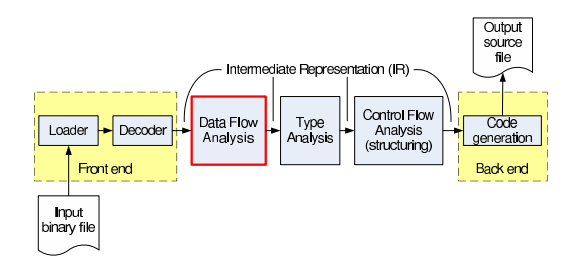
\includegraphics{fig32.png}
	\caption{Cấu trúc các khối lớn của Boomerang}
	\label{fig:boomstruct}
\end{figure}

Khi đọc vào một chương trình assembly, Boomerang sẽ lưu trữ chúng dưới cấu trúc sau:

\begin{figure}
	\centering
	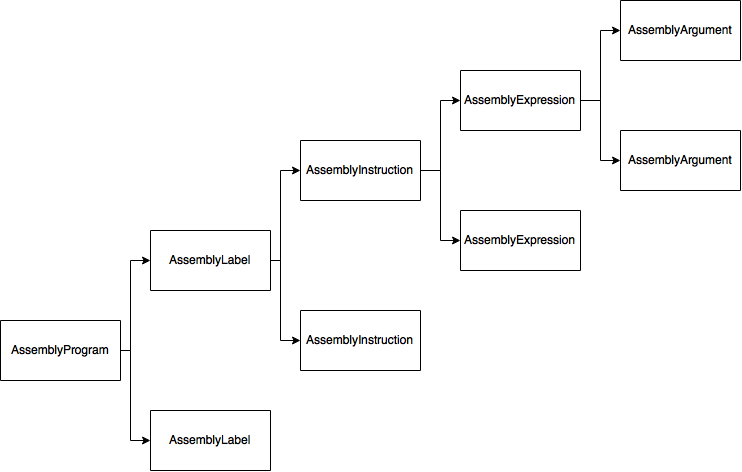
\includegraphics[width=0.7\linewidth]{assemblyInfo}
	\caption{Cấu trúc dữ liệu lưu trữ mã assembly trong Boomerang}
	\label{fig:assemblyinfo}
\end{figure}

Lưu ý, trong AssemblyArgument, giá trị thực sự của tham số được lưu vào một union có tên là Arg. Giá trị này có thể là một chuỗi (đối với trường hợp thanh ghi hoặc tên biến), một số nguyên, một số thực hoặc một structure đại diện cho bit (bao gồm tên thanh ghi và vị trí của bit).
\begin{lstlisting}[caption={Đoạn mã mô tả cách biểu diễn giá trị của tham số trong Boomerang}, label={}]
struct bits{
	char* reg;
	int pos;
}
union Arg{
	int i;
	float f;
	char* c;
	bits bit;
}
\end{lstlisting}

Khi giải mã lên ngôn ngữ trung gian, cấu trúc Boomerang dùng để thể hiện là:

\begin{figure}
	\centering
	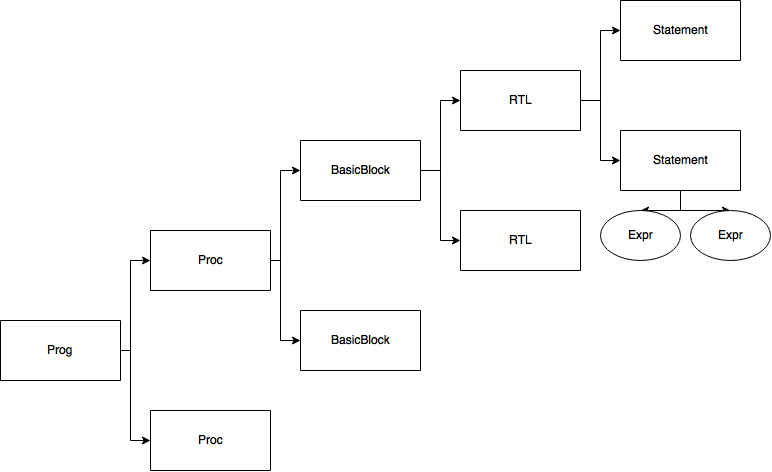
\includegraphics[width=0.7\linewidth]{progBoomerang}
	\caption{Cách lưu trữ một chương trình dưới dạng mã trung gian của Boomerang}
	\label{fig:progboomerang}
\end{figure}


Prog là tương ứng với toàn bộ chương trình. Một Proc là một hàm, BasicBlock đại diện cho một khối cơ bản mà ở đó không có một câu lệnh rẽ nhánh nào (ví dụ như if, hoặc vòng lặp...). Statement là một câu lệnh và Expr là các biểu thức trong chương trình. Ngoài ra còn có các class đại diện cho kiểu dữ liệu. Việc thực hiện các phân tích chủ yếu diễn ra tại Proc, vì vậy, các thay đổi trong luận văn này cũng chủ yếu được thực hiện bằng các hàm của Proc.\\

Như vậy, để thực hiện việc xử lý mã 8051, ta cần phải chỉnh sửa các phần sau đây của Boomerang:
\begin{itemize}
	\item Phần parser để chấp nhận câu lệnh \#DEFINE, cũng như lưu trữ biến và giá trị của biến vào một bảng dữ liệu.
	\item Phần giải mã từ mã assembly lên mã trung gian để đưa các biến không phải thanh ghi thành một biểu thức trung gian phù hợp.
	\item Phần chuyển đổi từ biểu thức trung gian thành tên biến để giải quyết các trường hợp biến không phải thanh ghi. Hiện tại, Boomerang chỉ cho phép người dùng định nghĩa sẵn một danh sách thanh ghi của kiến trúc máy và dựa vào đó để chuyển đổi. Cần có cơ chế để Boomerang có thể chuyển đổi các biến ngoài danh sách thanh ghi đó.
	\item Phần phân tích dữ liệu của Boomerang để thêm vào một phân tích hỗ trợ cho việc nhận biết các bộ biến. Mỗi giải pháp sẽ có một phương pháp phân tích khác nhau và được trình bày ở các chương kế.
\end{itemize}
Các thay đổi này sẽ được trình bày kỹ hơn ở mục \ref{sec:boomchange}.